\chapter{Photon diffusion approximation} \label{chap:stellarinterior}
\PartialToc



\section{Equazione di stato}

\subsection{Legge dei gas perfetti e stato di ionizzazione della materia stellare}

Nell'interno stellare si raggiunge rapidamente l'equlibrio su scala atomica ma non nucleare (steady macroscopic state: principles of statistical physics): rates of all atomic reactions equal those of their reverse.

Le funzioni che descrivono uno stato di equilibrio dipendono dalla composizione chimica (:$\mu$), $\rho$, T.

Una funzione $P=P(\rho,T)$ \'e la funzione di stato: struttural support against gravity.

Vicino alla superficie la funzione di stato \'e complicata dalla presenza di atomi parzialmente ionizzati.

Per $T\geq 10^5 K$ diventa viavia pi\'u esatto considerare il gas completamente ionizzato; the bulk of the structure of most stars is detemined by an equation of state for completely ionized matter. Completely ionized gas behave like perfect gas up to high densities: radii of nuclei are $10^{-5}$ those of atoms, a gas composed of nuclei and electrons occupies $\approx10^{-15}$ of the volume occupied by atoms.

In un gas perfetto le interazioni fra particelle sono trascurabili $E_{int}\approx\exv{E_{Cou}}\ll KT$ for non degenerate gas.


\begin{align*}
&n=\frac{N}{V}\\
&\rho=\frac{M}{V}\\
&m_0=\frac{M}{N}&\intertext{\'e il peso molecolare medio}\\
\end{align*}
ho l'equazione di stato
\begin{align*}
&PV=nRT=NKT&\intertext{Riscrivo l'equazione di stato esprimendo la pressione in funzione della densit\'a, temperatura e composizione}\\
&P=(\frac{N}{V})KT=nKT=\frac{\rho}{m_0}KT\\
&P=\frac{1}{\mu}\frac{K_B}{m_P}\rho T&\intertext{definisco il peso molecolare in termini di proton mass}\\
&\frac{1}{\mu}=2X+\frac{3}{4}Y+\frac{Z}{2}
\end{align*}

\begin{usefull}{Peso molecolare medio}

Equazione di stato per un gas di particelle materiali non-interacting non-degenerate

\begin{align*}
&P_g=nkT\\
&P_g=(\frac{\gasconstant{}}{\mu})\rho T&\intertext{dove $\gasconstant{}$ \'e in moli $\mu$ \'e il peso molecolare medio (massa per mole di particelle libere)}
\end{align*}

\begin{definition}{Peso molecolare medio}
Segue dalla definizione di mole che $\mu$, the total rest mass per mole of free particles is also equal to average rest mass in amu per free particles ($\si{\atomicmassunit}=\frac{1}{N_A}\approx M(H^1)$): $\mu$ depends on number of free particles contained in a fixed rest mass of the material (fixed value of the product of the number of free particles in the system and average rest mass per free particle).

\begin{align*}
&\mu=(\frac{\rho}{H})\frac{1}{n}=\frac{\sum_kA_kn_k}{\sum_kn_k}&\intertext{where}\\
&A_k=\frac{m_k}{H},\ n_k=\frac{\rho x_k}{HA_k}\\
&\mu=\frac{1}{\sum_k\frac{x_k}{A_k}}
\end{align*}

In case free electrons have been released by ionization of atoms
\begin{align*}
&n=n_e+\sum_in_i&\intertext{$n_e$ is the number density of ionization electrons. Sia $\nu_e(i)$ il numero medio di elettroni liberati da ionizzazione specie i:}\\
&n_e=\sum_i\nu_e(i)n_i=\frac{\rho}{H}\sum_i\nu_e(i)\frac{x_i}{A_i}\\
&n=\frac{\rho}{H}\sum_i[1+\nu_e(i)]\frac{x_i}{A_i}=\frac{\rho}{H}\sum_i\bar{n}_ix_i&\intertext{where $\frac{[1+\nu_e(i)]}{A_i}$ is what Chandra called ''mean ionization per unit atomic weight'': total number of free particle per unit atomic mass contributed by particles of type i and atomic weight $A_i$.}\\
&\bar{n}_H=\frac{2}{1.008}\approx2,\ \bar{n}_{He}=\frac{3}{4.004}\approx0.75\\
&\mu=\frac{1}{\sum_i\bar{n}_ix_i}&\intertext{Assuming heavier elements than He completely ionized (and $A_i\approx2Z_i$ so that $\bar{n}_i\approx\frac{1}{2}$ for ($Z_i>2$)):}\\
&\mu=\frac{1}{\bar{n}_HX+\bar{n}_{He}Y+\bar{n}_{Z}Z}\\
&\mu\approx\frac{1}{2X+\frac{3}{4}Y+\frac{1}{2}Z}&\intu{for complete ionization}
\end{align*}

\end{definition}

The process of ionization dissociation and nuclear reaction alter the number of free particles in a given mass of the gas.


\end{usefull}


\subsection{Composizione chimica: numero di particelle libere per unit\'a di volume e peso molecolare medio $\mu$}
\index{Peso molecolare: particelle libere. ???}
We want to relate number of free particles N to the density; ho le lettere standard per l'abbondanza degli elementi: $X+Y+Z=1$ e A peso atomico medio per elementi pi\'u pesanti dell'elio

\begin{tabular}{c|ccc}
Elements: & $^1H$ & $^4He$ & Heavier\\
\hline
 $\#$ atoms per $cm^3$ & $\frac{X\rho}{m_p}$ & $\frac{Y\rho}{4m_p}$ & $[\frac{Z\rho}{Am_p}]$\\
 $\#$ electrons per $cm^3$ & $\frac{X\rho}{m_p}$ & $\frac{2Y\rho}{4m_p}$ & $\frac{1}{2}A\frac{Z\rho}{Am_p}$
\end{tabular}

In a completely ionized gas the number of free particles per cubic centimeter is 
\begin{equation*}
N=(2X+\frac{3}{4}Y+\frac{1}{2}Z)\frac{\rho}{m_p}
\end{equation*}

L'equazione di stato dei gas perfetti diventa
\begin{align*}
P=\frac{1}{\mu}\frac{K_b}{m_p}\rho T\\
\frac{1}{\mu}=2X+\frac{3}{4}Y+\frac{1}{2}Z
\end{align*}

Definizioni alternative di peso molecolare medio

\begin{align*}
&\rho=n\mu m_u&\intertext{n particelle per unit\'a di volume con stesso peso molecolare $\uparrow$. In generale}\\
&n_i=\frac{\rho_i}{\mu_im_u}=\frac{\rho}{m_u}\frac{X_i}{\mu_i}&\intertext{e per atomi completamente ionizzati (nucleus + free electrons)}\\
&n=n_e+\sum_in_i=\sum_i(1+Z_i)n_i\tikzmark{first}\\
&P=nkT=R\sum_i(\frac{X_i(1+Z_i)}{\mu_i})\rho T\tikzmark{second}
\end{align*}


Atomo neutro e contributo elettroni liberi.

Per un gas composto da atomi neutri ho:

$\mu_0=(\sum_i\frac{X_i}{\mu_i})^{-1}$.

Per gas completamente ionizzati definisco il peso molecolare medio per elettroni liberi:

\begin{align*}
&\mu_e=(\sum_iX_iZ_i/\mu_i)^{-1}&\intertext{for elements heavier than helium $\frac{\mu_i}{Z_i}\approx2$}\\
&\approx(X+\frac{1}{2}Y+\frac{1}{2}(1-X-Y))^{-1}=\frac{2}{1+X}
\end{align*}


\subsection{Gas di fotoni}


In prima approssimazione in un interno stellare
\begin{align*}
&P=P_g+P_{rad}=\frac{R}{\mu}\rho T+\frac{a}{3}T^4\\
&P_{Rad}=\frac{1}{3}\int_0^{\infty}\frac{h\nu}{c}cn(\nu)\,d\nu\\
&=\frac{1}{3}U=\frac{a}{3}T^4&\intertext{$\uparrow$ \'e la densit\'a di energia e}\\
&a=7.56*10^{-15}\,erg\,cm^{-3}\,K^{-4}
\end{align*}

Misuro l'importanza della pressione di radiazione con il parametro $\beta$
\begin{align*}
&\beta=\frac{P_g}{P}\\
&1-\beta=\frac{P_{Rad}}{P}
\end{align*}
\index{Parametro beta}

\begin{definition}{Emission coefficient}
Let's consider small mass element m which is radiating: the amount of radiant energy emitted by solid angle $d\omega$, frequency interval $[\nu,\nu+d\nu]$ and time $dt$

\begin{equation*}
j_{\nu}m\,d\omega\,dt\,d\nu
\end{equation*}

$j_{\nu}$ is called emission coefficient for frequency $\nu$.

\end{definition}



\subsection{Einstein coefficient.}

\begin{definition}{Spontaneous/induced emission coefficient.}

The probability that an atom in an excited state n emits in direction $d\omega$ and time $dt$ quanta of energy $h\nu_{nm}$ in absence of sxternal field is
\begin{equation*}
    A_{nm}\,d\omega\,dt
\end{equation*}

In presence of external field of radiation of intensity $I_{\nu_{nm}}$
\begin{equation*}
B_{nm}I_{\nu_{nm}}\,d\omega\,dt
\end{equation*}

\end{definition}

\subsection{Thermodynamical equilibrium.}

\subsection{Radiative equilibrium.}

La pressione di radiazione agisce a tutti gli effetti come una pressione cio\'e il suo gradiente \'e una forza 
\begin{align*}
&[H]=\text{Net energy transport/$cm^2$/s}\\
&F_{Rad}=\kappa_{\rho}H\frac{1}{c}\\
&F_{Rad}=-\frac{d}{dr}(\frac{a}{3}T^4)=-\frac{dP_R}{dr}
\end{align*}



\section{Adiabatic processes}

Most of the gas in a star can be thought as adiabatic: any process that take place on a timescale shorter than $\tkh{}$ can be thought of as adiabatic.

\begin{align*}
&\TDy{t}{u}+P\TDof{t}\frac{1}{\rho}=\epsilon-\TDy{m}{F}=0&\intertext{and for many types of gas $u=\phi\frac{P}{\rho}$ quindi}\\
&\frac{dP}{P}=(\frac{\phi+1}{\phi})\frac{d\rho}{\rho},\ \ln{P}=\gamma_a\ln{\rho}+\ln{K_a}&\intertext{the constant $K_a$ is determined by the entropy of the gas}
\end{align*}

All monoatomic ideal gas have $\gamma_a=\frac{5}{3}$, all relativistic gasses have $\gamma_a=\frac{4}{3}$.

Nel caso $K_a$ sia costante, tipo nella zone convettive, posso usare una relazione politropica con $\gamma_P=\gamma_a$.

\begin{usefull}{Difference polytropic relation vs adiabatic exponent}

\begin{itemize}
\item Polytropic relation describes how pressure change with density inside as one moves through the star.
\item Adiabatic equation of state describe how how a given gas shell would respond to being compressed.
\end{itemize}

\end{usefull}


\section{Ionizzazione}

\subsection{Idrogeno}
Definisco il grado di ionizzazione ($x=1$ per gas completamente ionizzato, $x=0$ per gas neutro)
\begin{equation*}
x=\frac{n_1}{n_0+n_1},\quad\frac{n_1}{n_0}=\frac{x}{1-x}
\end{equation*}
\index{Grado di ionizzazione: $^1H$}

Equazione di Saha
\begin{align*}
&\frac{n_{r+1}}{n_r}P_e=\frac{xP_e}{1-x}\\
&P_e=\frac{x}{1+x}P_{Gas}\\
&\frac{x^2}{1-x^2}=K_H\\
&K_H=\frac{u_1}{u_0}\frac{2}{P_{Gas}}\frac{(2\pi m_e)^{\frac{3}{2}}}{h^3}(KT)^{\frac{5}{2}}\exp{-\frac{\chi_H}{KT}}\\
&\chi_H=13.6\, eV
\end{align*}

Nella fotosfera (cgs) \mblock{P_{Gas}=6.83*10^4,\ T=5636\,K}: $x=10^{-4}$.

Deep layer (cgs) \mblock{P_{Gas}=1.56*10^{12},\ T=7.15*10^5\,K}: $x=0.993$.

Comportamento di $K_H$ in funzione di T e $P_{Gas}$:

aumenta con T e decresce con la pressione e stessa cosa per il grado di ionizzazione. Infatti con T aumenta anche l'energia delle collisioni e dei fotoni, mentre all'aumentare di $P_{Gas}$ aumenta la probabilit\'a di ricombinazione elettroni/ioni.

Determino $\mu$ per gas di idrogeno con grado di ionizzazione x: $\mu m_u$, $\mu_0m_u$, $\mu_em_u$ sono definiti come masse medie per, rispettivamente, particelle libere,  nuclei ed elettroni liberi.

Numero di elettroni liberi per atomo: \mblock{E=\frac{n_e}{n}=x}.
\begin{align*}
\rho=(n+n_e)\mu m_u=n\mu_0m_u=n_e\mu_em_u&\intertext{Usando $n=n_0+n_1$, risolvo per $\mu$: $\downarrow$}\\
\mu=\frac{\rho}{m_un}\frac{1}{1+x}=\frac{\mu_0}{1+x}=\mu_e\frac{x}{1+x}&\intertext{$\uparrow$ \'e valida per miscela di gas salvo che $E\neq x$}
\end{align*}
\index{Mean molecular weight for partially ionized hydrogen}

\subsection{H-He mixture}

Ho un gas di idrogeno ed elio di abbondanze relative X e Y: 3 energie di ionizzazione per idrogeno neutro $\chi_H^0=13.6\,eV$ e $\chi_{He}^0=24.6\,eV$, $\chi_{He}^1=54.4\,eV$ per elio neutro e 1-ionizzato.

Contributi energia interna atomi ionizzati.
\begin{itemize*}
\item Ogni atomo di idrogeno ionizzato contribuisce $\chi_H^0$.
\item Ogni atomo di He ionizzato 1 volta contribuisce $\chi_{He}^0$
\item Ogni atomo di He privo di elettroni $\chi_{He}^0+\chi_{He}^1$
\end{itemize*}

Definisco il grado di ionizzazione $x_i^r$ (il numero di atomi di tipo i ionizzati r diviso il numero totale di atomi i):
\begin{align*}
&x_H^0=\frac{n_H^0}{n_H},\quad x_H^0=\frac{n_H^1}{n_H}\\
&x_{He}^0=\frac{n_{He}^0}{n_{He}},\quad x_{He}^1=\frac{n_{He}^1}{n_{He}},\quad x_{He}^2=\frac{n_{He}^2}{n_{He}}
\end{align*}

Contributo dell'energia di ionizzazione all'energia interna
\begin{align*}
&u_{ion}=\frac{1}{m_u}\{Xx_H^1\chi_H^0\\
&+\frac{1}{4}Y[x_{He}^1\chi_{He}^0+x_{He}^2(\chi_{He}^0+\chi_{He}^1)]\}&\intertext{$\frac{X}{m_u}$ \'e il numero di atomi d'idrogeno, $\frac{Y}{4m_u}$ \'e il numero di atomi di elio}
\end{align*}

Ho 3 equazioni di Saha: 6 equazioni per sei incognite $x_H^0$, $x_H^1$, $x_{He}^0$, $x_{He}^1$, $x_{He}^2$, $E$.

\begin{align*}
&\frac{x_H^1}{x_H^0}\frac{E}{E+1}=K_H^0\\
&\frac{x_{He}^1}{x_{He}^0}\frac{E}{E+1}=K_{He}^0\\
&\frac{x_{He}^2}{x_{He}^1}\frac{E}{E+1}=K_{He}^1&\intertext{$\uparrow$ equazioni di Saha: sono occoppiate tra loro tramite $E$. Inoltre:}\\
&E=[Xx_H^1+\frac{1}{4}Y(x_{He}^1+2x_{He}^2)]\mu_0\\
&K_i^r=\frac{u_{r+1}}{u_r}\frac{2}{P_{Gas}}\frac{(2\pi m_e)^{\frac{3}{2}}(KT)^{\frac{5}{2}}}{h^3}\exp{-\frac{\chi_i^r}{KT}}\\
&x_H^0+x_H^1=1,\quad x_{He}^0+x_{He}^1+x_{He}^2=1
\end{align*}


\chapter{Ionized real gas}
\PartialToc

\section{Grandezze termodinamiche di un plasma classico}

\subsection{Passoggio da unit\'a energetiche a gradi (Landau)}

\begin{align*}
&k=\SI{1.38e-16}{\erg\per\kelvin},\ \SI{1}{\ev}=\SI{11606}{\kelvin}\\
&S=k\ln{\Delta\Gamma}\\
&T\to kT,\ S\to\frac{S}{k}
\end{align*}

\subsection{Sviluppo in serie di potenze della  densit\'a per un gas neutro}

Considero il gas abbastanza rarefatto in modo da poter trascurare le collisioni che coinvolgono pi\'u di 2 atomi/molecole. Per un gas monoatomico reale classico l'energia si scrive \mblock{E(p,q)=\sum^N\frac{p_a^2}{2m_a}+U} e $U$ \'e l'energia di interazione tra gli atomi.

\begin{align*}
&F=-kT\ln{\int\exp{-\frac{E(p,x)}{kT}}\,d\Gamma}&\intertext{considerando anche le interazioni}\\
&F=F_{perf}\\
&-kT\ln{\frac{1}{V^N}}\int d^3p_1\ldots\,d^3p_N\int\exp{-\frac{U}{kT}}d^3x_1\ldots\,d^3x_N\\
&F=F_{perf}\\
&+\frac{N^2TB(T)}{V},\ B(T)=\frac{1}{2}\int(1-\exp{-\frac{U_{12}}{kT}})\,d^3x&\intertext{da cui trovo la pressione e quindi l'equazione di stato aanell'approssimazione considerata}\\
&P=-\PDy{V}{F}=\frac{NkT}{V}(1+\frac{NB(T)}{V})
\end{align*}

Lo sviluppo in serie di potenze di $\frac{1}{V}$ \'e
\begin{equation*}
P=\frac{NkT}{V}(1+\frac{NB(T)}{V}+\frac{N^2C(T)}{V^2}+\ldots)
\end{equation*}

B, C sono il secondo e il terzo coefficiente del viriale.

Per determinare questi coefficienti considero il potenziale
\begin{align*}
&\exp{-\frac{\Omega}{kT}}=\sumzi{N}\frac{1}{N!}\exp{\frac{\mu N}{kT}}\int \exp{-\frac{E_N(p,x)}{kT}}\,d\Gamma_N\\
&E_3(p,x)=\sum\frac{p_a^2}{2m_a}+U_{123}
\end{align*}

\subsection{Gas completamente ionizzato}

Per calcolare le correzioni di un gas di particelle interagenti tramite forza coulombiana \'e necessario sviluppare una tecnica diversa da quella dello sviluppo in termini del viriale per gas di particelle neutre.

Considero il gas completamente ionizzato e globalmente neutro: \mblock{\sum_az_aeN_{a0}}. Supponiamo che il gas devii dallo stato perfetto: \'e indispensabile che l'energia coulombiana media tra due ioni \mblock{\frac{(ze)^2}{\overline{r}}}, con \mblock{\overline{r}\approx r\expy{-\frac{1}{3}}} distanza media tra gli ioni, sia piccola rispetto all'energia cinetica $kT$:
\begin{align*}
&(ze)^2n\expy{\frac{1}{3}}\ll kT\\
&n\ll(\frac{kT}{z^2e^2})^3 
\end{align*}

Poich\'e il plasma \'e elettricamente neutro il valore medio dell'energia di interazione coulombiana tra le particelle se fossero uniformemente distribuite in maniera indipendente si annullerebbe.

\begin{definition}{Correzione correlative delle grandezze termodinamiche}

Le prime correzioni alle grandezze termodinamiche del plasma rispetto al gas perfetto compaiono se si tiene conto delle correlazioni tra le diverse particelle.

\end{definition}

Per la correzione all'energia coulombiana del plasma $E_{cor}$ scrivo l'energia di interazione elettrostatica di un sistema di particelle cariche come

\begin{equation*}
E_{cor}=V\frac{1}{2}\sum_aez_an_{a0}\phi_a
\end{equation*}

dove $\phi_a$ \'e il potenziale creato dalle altre particelle cariche e agente sullo ione dell'a-esimo tipo.

Ciascuno ione crea attorno a se una nube ionica a simmetria sferica: indicando con $n_a$ la densit\'a degli ioni dell'a-esimo tipo in questo nube ionica, l'energia potenziale di ciascuno ione dell'a-esimo tipo nel campo esistente attorno al dato ione \'e $ez_a\phi$ dove $\phi$ \'e il potenziale del campo. In accordo con la formula di Boltzmann abbiamo
\begin{equation*}
n_a=n_{a0}\expp{(-\frac{z_ae\phi}{kT})}
\end{equation*}

il coefficiente costante si \'e posto $n_{a0}$ poich\'e lontano dal centro \mblock{\phi\to0} la densit\'a della nube ionica diventa la densit\'a media del gas.

Il potenziale $\phi$ del campo elettrico nella nube ionica \'e legato alla densit\'A di cariche, \mblock{\sum ez_an_a}, dall'equazione di Poisson

\begin{equation*}
\nabla^2\phi=-4\pi e\sum_az_an_a
\end{equation*}

Le ultime due equazioni definiscono il campo elettrico autocompatibile di elettroni e ioni.

Vista l'ipotesi di piccola energia di interazione tra gli ioni posso espandere gli esponenziali al termine lineare nel campo elettrico:

\begin{align*}
&\nabla^2\phi-\kappa^2\phi=0\\
&\kappa^2=\frac{4\pi e^2}{kT}\sum_an_{0a}z_a^2
\end{align*}

$\kappa$ \'e l'inverso di una lunghezza e la soluzione a simmetria sferica dell'equazione precedente \'e 
\begin{equation*}
\phi\propto\frac{\exp{-\kappa r}}{r}\\
\phi=ez_b\frac{\exp{-\kappa r}}{r}
\end{equation*}
la costante moltiplicativa si ha considerando che il potenziaöe per piccole distanze dal centro \'e $\frac{ez_b}{r}$. Il campo diventa molto piccolo a distanze grandi rispetto a $\frac{1}{\kappa}$.

\begin{definition}{Raggio di Debye}

La lunghezza \mblock{\frac{1}{\kappa}=\sqrt{\frac{kT}{4\pi e^2\sum_zz^2\overline{n}_z}}}.

\end{definition}

L'approssimazione di interazione debole \'e equivalente alla condizione che il raggio di Debye sia molto pi\'u grande della distanza media tra gli ioni.

Sviluppando il potenziale autocompatibile
\begin{equation*}
\phi=\frac{ez_b}{r}-ez_b\kappa+\ldots
\end{equation*}
i termini omessi si annullano per $r=0$. Il primo termine \'e il campo coulombiano dello ione in esame, il secondo \'e il campo creato da tutti gli altri ioni della nube nel punto in cui si trova lo ione dato quindi
\begin{align*}
&E_{cor}=V\frac{1}{2}\sum_aez_an_{a0}\phi_a&\intertext{sostituendo $\phi_a=-ez_a\kappa$}\\
&E_{cor}=-\frac{V}{2}\kappa e^2\sum_an_{a0}z_a^2=-Ve^3\sqrt{\frac{\pi}{kT}}(\sum_an_{a0}z_a^2)\expy{\frac{3}{2}}
\end{align*}

Dalla relazione termodinamica
\begin{align*}
&E=F-T\Dcvar{\PDy{T}{F}}{V}=-T^2\Dcvar{\PDof{T}\frac{F}{T}}{V}&\intertext{e ponendo la costante di integrazione uguale a zero poich\'e \mblock{F\abc{T\to +\infty}F_{perf}}}\\
&F=F_{perf}-\frac{2e^3}{3}\sqrt{\frac{\pi}{kTV}}(\sum_aN_az_a^2)\expy{\frac{3}{2}}&\intertext{ponendo $N_a=n_{a0}V$.}
\end{align*}

e per la pressione:

\begin{align*}
&P=_\Dcvar{\PDy{V}{F}}{T}\\
&P=\frac{NkT}{V}-\frac{e^3}{3V\expy{\frac{3}{2}}}\sqrt{\frac{\pi}{kT}}(\sum_aN_az_a^2)\expy{\frac{3}{2}}
\end{align*}

\section{Real ionized gas: coulomb pressure}


In presence of forces tbhe internal energy of mono-atomic gas must include potential energy of interaction
\begin{equation*}
E_i=\sum\frac{p^2}{2m}+\Phi
\end{equation*}
where $\Phi$ is the potential energy, depends upon interparticle distance and so upon density.

\subsection{Nearly perfect gas at low density: \mblock{n_Z\ll(\frac{kT}{Z^2e^2})^3}.}

The pressure is given by change in internal energy $dE_i$ associated with adiabatic compression \mblock{\Dcvar{dE_i}{ad}=-P\,dV}: if the internal energy is density dependent because of icoulomb interaction a pressure arises.

The Coulomb energy per unit volume is
\begin{equation*}
\Dcvar{\frac{U}{V}}{c}=\frac{1}{2}\sum_ZeZ\overline{n}_Z\Phi_Z
\end{equation*}



Riscrivo il raggio di Debye utilizzando il coefficiente $\zeta$
\begin{align*}
&\sum_ZZ^2\overline{n}_Z=\sum_Z(Z^2+Z)\overline{n}_Z=\sum_Z(Z^2+Z)\frac{\rho X_Z}{A_Z}N_A\\
&R_D=\sqrt{\frac{kT}{4\pi e^2\rho N_A\xi}}&\intertext{dove ho definito}\\
&\xi=\sum_{+Z}(Z^2+Z)\frac{X_Z}{A_Z}\\
\end{align*}
da cui l'energia potenziale coulombiana per unit\'a di volume:
\begin{align*}
&\Dcvar{\frac{E_i}{V}}{c}=-e^3\sqrt{\frac{\pi}{kT}}(\sum\overline{n}_ZZ^2)\expy{\frac{3}{2}}\\
&=-e^3\sqrt{\frac{\pi}{kT}}(\rho N_A\xi)\expy{\frac{3}{2}}
\end{align*}


Il procedimento di DH \'e valido se:
\begin{equation*}
\frac{3}{2}kT\frac{\rho N_A}{\mu}\gg\Dcvar{\frac{E_i}{V}}{coul}
\end{equation*}

\subsubsection{Coulomb pressure}

L'energia potenziale coulombiana per grammo \'e
\begin{equation*}
u_c=-e^3\sqrt{\frac{\pi\rho}{kT}}(N_A\xi)\expy{\frac{3}{2}}=\frac{B}{\sqrt{VT}}
\end{equation*}

Indicando il numero di particelle in \SI{1}{\gram} esprimo
\begin{align*}
&u=\frac{3}{2}kTN+u_c\\
&P=\frac{N}{V}kT+P_c
\end{align*}

La variazione infinitesima di entropia si scrive
\begin{align*}
&dS=\frac{1}{T}[\Dcvar{\PDy{V}{U}}{T}+P]\,dV+\frac{1}{T}\Dcvar{\PDy{T}{U}}{V}\,dT\\
&\Dcvar{\PDy{V}{U}}{T}=\Dcvar{\PDy{V}{U_c}}{T}=-\frac{1}{2}\frac{B}{V\expy{\frac{3}{2}}T\expy{\frac{1}{2}}}\\
&\Dcvar{\PDy{T}{U}}{V}=\frac{3}{2}Nk-\frac{1}{2}\frac{B}{V\expy{\frac{1}{2}}T\expy{\frac{3}{2}}}
\end{align*}

la condizione di integrabilit\'a su $dS$ richiede \mblock{\PDof{T}\frac{P_c}{T}=-\frac{1}{2}\frac{B}{V\expy{\frac{3}{2}}T\expy{\frac{5}{2}}}} che integrata da
\begin{equation*}
\frac{P_c}{T}=\frac{1}{3}\frac{B}{V\expy{\frac{3}{2}}T\expy{\frac{3}{2}}}+f(V)
\end{equation*}

e infine

\begin{equation*}
P_c=\frac{1}{3}\Dcvar{\frac{E_i}{V}}{c}=-\frac{e^3}{3}\sqrt{\frac{\pi}{kT}}(\rho N_A\xi)\expy{\frac{3}{2}}
\end{equation*}

\begin{exercise}{Coulomb and perfect gas pressure for He gas}

Compute Coulomb and perfect gas pressure for He gas at \mblock{T=\SI{e6}{\kelvin},\ \rho=\SI{e-2}{\gram\per\cubic\cm}}.

(Ans:\mblock{P_c=\SI{-4.8e9}{\dyn\per\square\cm},\ P_g=\SI{6.3e11}{\dyn\per\square\cm}})

\end{exercise}

\subsubsection{Depression of the continuum and effective ionization potential}

From \debh{} model the average potential around each electron is
\begin{equation*}
V_e(r)=-\frac{e}{r}+e\kappa-\ldots
\end{equation*}

so that the potential energy of each free electron due to interactions with other charges is \mblock{(PE)_e=-e^2\kappa=-\frac{e^2}{R_d}}: the negative energy reflects the fact that free electrons are bound to plasma as a whole. The energy of a zero kinetic energy electron is \mblock{E=-\frac{e^2}{R_D}} and one says that the continuum of states has been depressed.

The energy necessary to ionization is further reduced by changes in energies of bound states: the electrons moves in a shilded potential rather than in pure coulomb $\frac{1}{r}$, for a single bound electron the ground state radius is mach less than $R_D$ thus the electron buond to charge Z moves in a potential
\begin{equation*}
V(r)\approx\frac{Ze}{r}-\frac{/Z-1)e}{R_D}
\end{equation*}

where the second term is the potential due to the Debye sphere of charge $(Z-1)$ surrounding the ion. The potential energy of bound electron is
\begin{equation*}
(PE)_e\approx-\frac{Ze^2}{a}+\frac{(Z-1)e^2}{R_D}
\end{equation*}
where a is the radius of the orbital (for hydrogen-like atom: \mblock{a=\frac{a_0}{Z}}).

\begin{usefull}{Effective ionization potential}
\begin{equation*}
\chi_Z'=\chi_Z-\frac{Ze^2}{R_D}
\end{equation*}
\end{usefull}

\begin{exercise}{Partition function of five-times-ionized carbon atom}
A five times ionized carbon atom (H like) is embedded in H gas at \mblock{T=\SI{5e5}{\kelvin},\ \rho=\SI{5e-3}{\gram\per\cubic\cm}}. Estimate the partition function and how much the ionization energy of \SI{36}{\ryd} is reduced.

(\mblock{G_c=2.6,\ \Delta\chi\approx-1.0\si{\ryd}})
\end{exercise}

\subsection{Zero T}

\chapter{Reazioni nucleari}
\PartialToc


\section{PP cycle}

Nell'interno stellare l'idrogeno \'e ionizzato quindi nel caso di emissione di positroni nel Q-valore \'e compreso un contributo per l'annichilamento \Pelectron\APelectron.

\subsection{Bottle-neck}

\begin{align*}
&^1H+^1H\to^2H+\APelectron+\Pnue (Q=1.44 MeV)&\intertext{Il neutrino ha spettro continuo con endpoint}\\
&E(\nu)=0.42 MeV
\end{align*}

Reazione lenta:

\begin{align*}
&\sigma\approx 10^{-33}b (KeV)\\
&\approx 10^{-23} b (MeV)\\
&R=\frac{1}{2}n_P^2\exv{\sigma v}\approx5*10^{-18} \text{reazioni}/\text{P}/s\\
&\rhosunc=125gr/cm^3 \quad (7.5*10^{25}P/cm^3)\\
&\tsunc 15*10^6K\Rightarrow\exv{T_P}\approx1 KeV&
\intertext{per le regioni centrali del sole.}
\end{align*}

\subsection{Deuteron cooking up to Helium}

Il deutone viene trasformato rapidamente in isotopo di elio
\begin{equation*}
^2H+^1H\to \indices{^3}He+\gamma \quad (Q=5.49 MeV)
\end{equation*}

\subsection{Produzione di He4: ciclo PP1 (Sun: \mblock{69\%}).}
\begin{equation*}
^3He+^3He\to^4He+2^1H+\gamma\quad(Q=12.86 MeV)
\end{equation*}

\subsection{Bilancio energetico PP}
L'energia dei neutrini che escono dal core non scalda la fotosfera.
\begin{align*}
Q=26.7 MeV &\intertext{Atomi neutri e annichilamento \Pelectron\APelectron.}
\end{align*}

\subsection{Tempi medi di reazione nella catena PP.}
Per le condizioni presenti nel sole:

\begin{tabular}{|c|c|}
\hline
Reazione & $t_r$ \\
\hline
$^1H+^1H\to^2H+\APelectron+\Pnue$ & $7*10^9\,yr$\\
$^2H+^1H\to ^3He+\gamma$ & $4 s$\\
$^3He+^3He\to^4He+2^1H$ & $4*10^5\,yr$\\
$^{12}C+^1H\to ^{13}N+\gamma$ & $10^6\, yr$\\
$^{13}N\to^{13}C+\APelectron+\Pnue$ & $10\,min$\\
$^{13}C+^1H\to ^{14}N+\gamma$ & $2*10^5\, yr$\\
$^{14}N+^1H\to ^{15}O+\gamma$ & $<3*10^7\, yr$\\
$^{15}O\to^{15}N+\APelectron+\Pnue$ & $2\,min$\\
$^{15}N+^1H\to ^{12}C+^4He$ & $10^4\, yr$\\
\hline
\end{tabular}

\section{Altre diramazioni della catena \Pproton\Pproton dopo produzione He3.}

\subsection{Ciclo HeP (Sun: $0.0001\%$).}
\begin{align*}
&^3He+^1H\to^4He+\APelectron+\Pnue \quad (Q=19.28 MeV)\\
&E_{\nu}^{max}=Q-m_ec^2=18.77 MeV
\end{align*}

\subsection{Produzione Be7 (Sun: $31\%$).}
\begin{equation*}
^3He+^4He\to^7_4Be+\gamma
\end{equation*}
da cui seguono 2 diramazioni:

\subsection{Ciclo PP2 (Sun: $99.7\%$).}
\begin{align*}
^7_4Be+\Pelectron\to^7_3Li+\Pnue&\intertext{CE: decadimento a 2 corpi: neutrino monoenergetico}\\
E(\nu)\approx0.862 MeV\\
^7_3Li+^1H\to2^4He
\end{align*}

\subsection{Ciclo PP3 (Sun: $0.3\%$).}
\begin{align*}
^7_4Be+^1H\to^8_5B+\gamma\\
^8_5B\to^8_4Be+\APelectron+\Pnue&\intertext{Spettro energetico del neutrino continuo con endpoint}\\
E(\nu)=14 MeV\\
^8_4Be\to2^4He
\end{align*}

\subsection{Energia irradiata in neutrini}
\begin{align*}
Q_{eff}&=Q-\exv{E_{\nu}}(MeV)\quad&\text{Perdita in neutrini}&\intertext{PP1}\\
&=26.2 &2\%&\intertext{PP2}\\
&=25.66  & 4\%&\intertext{PP3}\\
&=19.17  & 28\%
\end{align*}


\section{Ciclo CNO}
Procede con maggiore velocit\'a perch\'e non \'e presente il bottleneck $H+H\to D$ ma la barriera coulombiana per la fusione dei nuclei \'e 6-7 volte pi\'u elevata: efficiente ad alte temperature.

\begin{figure}[!ht]
\centering
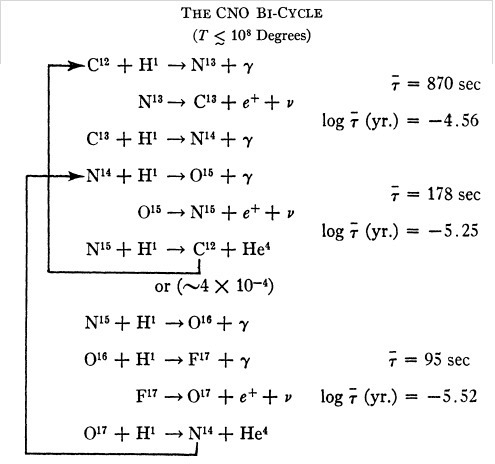
\includegraphics[width=(\textwidth),height=(\textheight-11mm),keepaspectratio]{cnobi}
\caption{Bi-ciclo CNO.}
\end{figure}

\begin{align*}
^{12}_6C+^1H\to^{13}_7N+\gamma\\
^{13}N\to ^{13}_6C+\APelectron+\Pnu\\
^{13}C+^1H\to ^{14}_7N+\gamma\\
^{14}_7N+^1H\to ^{15}_8O+\gamma\\
^{15}_8O\to ^{15}_7N+\APelectron+\gamma\\
^{15}_7N+^1H\to ^{12}_6C+^4_2He
\end{align*}

Processo efficace:

$4^1H\to ^4He+2\APelectron+2\Pnue$ uguale alla catena PP, stesso Q-valore.

\clearpage



\chapter{Strutture degeneri}
\PartialToc

\section{Degenerazione}

Il sole \'e descrivibile con equazioni non degeneri le nane bianche con equazioni degeneri.

\subsection{Electron's degeneracy}
The degeneracy is due to Pauli exclusion principle for electron rather than gas density approaching nuclear densities: $\rho_N\approx10^{12}g/cm^3$ which is more than a factor $10^3$ higher than the highest densities we will encounter.

\begin{equation*}
n_E\,d^3p_e\,d^3x\leq\frac{2}{h^3}\,d^3p_e\,dV
\end{equation*}

If we put more electrons in our small space volume the maximum of distribution function will soon approach the ceiling.

\subsection{Complete degeneracy}

Derivo l'equazione di stato per un gas completamente degenere: determino pressione e densit\'a.

Relazione tra impulso di Fermi e densit\'a.

\begin{align*}
&N_E=\frac{1}{V}\int_{|p|=0}^{|p|=p_0}\frac{2}{h^3}\,d^3p\,d^3x=\frac{2}{h^3}\frac{4\pi}{3}p_0^3\\
&N_E=\frac{1}{\mu_E}\frac{\rho}{m_p},\quad\frac{1}{\mu_E}=X+\frac{1}{2}Y+\frac{1}{2}Z\\
&=\frac{1}{2}(1+X)&\intertext{Risolvendo le ultime 2 equazioni ricavo la densit\'a in funzione dell'impulso di Fermi}\\
&\frac{1}{\mu_E}\rho=\frac{8\pi}{3}\frac{m_P}{h^3}p_0^3\\
\end{align*}

Relazione tra impulso di Fermi e pressione.

\begin{align*}
&P_E=\int_{|p|=0}^{|p|=p_0}p_xv_x\frac{2}{h^3}\,d^3p&\intertext{$\uparrow$ is rate of transport of momentum: the momentum $p_x$ of a cubic centimeter transported through a square centimeter at rate given by $v_x$. That here we have singled out the x direction is of no consequence since the momentum distribution is spherical.}\\
&P_E=\frac{8\pi}{15mh^3}p_0^5&\intertext{$\uparrow$ espressione per velocit\'a non relativistiche: ho usato $v_x=\frac{p_x}{m}$.}\\
&P_E=\frac{2\pi c}{3h^3}p_0^4&\intertext{$\uparrow$ espressione per velocit\'a relativistiche: ho usato $v_x=c\frac{p_x}{|p|}$.}
\end{align*}

Equazione di stato.
\begin{align*}
&P_E=K_{NR}(\frac{1}{\mu_E}\rho)^{\frac{5}{3}}&\intertext{$\uparrow$ equazione di stato per gas di elettroni completamente degenere non relativistico, }\\
&K_{NR}=\frac{h^2}{20m_em_p}(\frac{3}{\pi m_p})^{\frac{2}{3}}=9.91*10^{12}\\
&P_E=K_R(\frac{1}{\mu_E}\rho)^{\frac{4}{3}}&\intertext{$\uparrow$ equazione di stato per gas di elettroni completamente degenere relativistico, }\\
&K_R=\frac{hc}{8m_p}(\frac{3}{\pi m_p})^{\frac{1}{3}}=1.23*10^{15}
\end{align*}

La pressione totale \'e $P=P_A+P_E$ dove $P_A$ \'e data dall'equazione dei gas perfetti: all'equilibrio termico gli atomi hanno la stessa energia per particella degli elettroni quindi data la maggiore massa hanno un momento maggiore di $\sqrt{\frac{m_A}{m_E}}$ e occupano un volume nello spazio dell fasi $(\frac{m_A}{m_E})^{\frac{3}{2}}$ maggiore degli elettroni: gli atomi hanno a disposizione un volume dello spazio delle fasi $10^5$ volte maggiore degli elettroni.

\section{Region in diagram density-temperature and equation of state}

\begin{figure}[!ht]
\centering
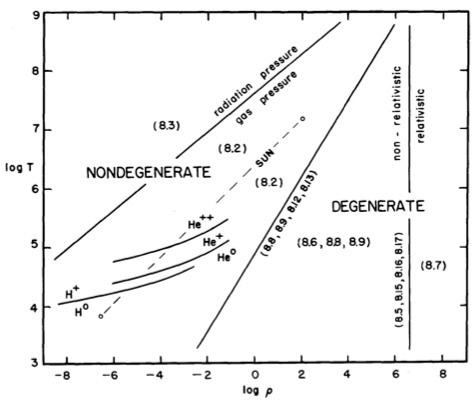
\includegraphics[width=(\textwidth),height=(\textheight-11mm),keepaspectratio]{Trho-state}
\caption{Equazione di stato nel diagramma densit\'a-Temperatura.}
\end{figure}

\subsection{Degeneracy limits}
Cerco il confine nel diagramma temperatura-densit\'a fra regione degenere e non-degenere e, nella regione degenere tra la parte relativistica e non relativistica.

Definisco il limite tra le regione degenere/non-degenere attraverso l'uguaglianza
\begin{align*}
\frac{1}{\mu_E}\frac{K}{m_P}\rho T=K_{NR}(\frac{1}{\mu_E}\rho)^{\frac{5}{3}}&\intertext{Risolvendo $\uparrow$ per la densit\'a:}\\
\frac{1}{\mu_E}\rho=(\frac{KT}{m_PK_{NR}})^{\frac{3}{2}}=2.4*10^{-8}T^{\frac{3}{2}}
\end{align*}

e il confine tra regione non-relativistica e relativiastica uguagliando la pressione data delle risp. formule
\begin{equation*}
\frac{1}{\mu_E}\rho=(\frac{K_R}{K_{NR}})^3=1.916*10^6
\end{equation*}

\subsection{Radiation/gas pressure limit}

The upper left corner represent the region where radiation pressure is dominant. The boundary line represents the equation \mblock{P_{Rad}=P_G}.

Throughout the majority of stars radiation pressure is of no importance.


\section{Electron degeneracy}

\subsection{Boltzmann statistic}

High density in volume $dV$ so that is fully pressure ionized: free electron of density $n_e$. If the velocity distro is given by Boltzmann statistic their mean kinetic energy is \mblock{\frac{3kT}{2}}: the number of electrons in spherical shell $[p,p+dp]$ is
\begin{equation*}
f(p)\,dp\,dV=n_e\frac{4\pi p^2}{(2\pi m_ekT)\expy{\frac{3}{2}}}\exp{-\frac{p^2}{2m_ekT}}\,dp\,dV
\end{equation*}

A reduction of $T$ with $n_e$ constant cause maximum of distro function $p_{max}=\sqrt{2m_ekT}$ to tends to smaller values of $p$ and the maximum of $f(p)$ becomes higher since \mblock{n_e=\intzi f(p)\,dp}

\subsection{Pauli principle}

Each quantum cell of 6D phase space can't contain more than 2 electrons with \mblock{d^3pdV=h^3}: in the shell \mblock{[p,p+dp]} of momentum space there are \mblock{4\pi p^2\,dp\,dV/h^3} quantum cells which can't contain more than \mblock{2*4\pi p^2\,dp\,dV/h^3}:
\begin{equation*}
f(p)\,dp\,dV\leq2*4\pi p^2\,dp\,dV/h^3
\end{equation*}

The Boltzmann distro for $n_e$ constant is in contraddiction with QM for low T.

\subsection{Complete degeneracy: T=0.}

The state in which all electrons have lowest energy without violating PP is that in which all phase cells are occupied up to $p_F$
\begin{align*}
&f(p)=\frac{8\pi p^2}{h^3}\ p\leq p_F\\
&f(p)=0\ p\geq p_F
\end{align*}

quindi
\begin{align*}
&n_e\,dV=dV\int_0^{p_F}\frac{8\pi p^2\,dp}{h^3}=\frac{8\pi}{3h^3}p_F^3\,dV:\\
&p_F\propto n_e\expy{\frac{1}{3}}&\intertext{non relativistic:}\\
&E_F=\frac{p_F^2}{2m_e}\propto n_e\expy{\frac{2}{3}}
\end{align*}

If density is high enough we can have velocity comparable to $c$:

\begin{align*}
&p=\frac{m_ev}{\sqrt{1-v^2/c^2}}\\
&E_{tot}=\frac{m_ec^2}{\sqrt{1-v^2/c^2}}=m_ec^2\sqrt{1+\frac{p^2}{m_e^2c^2}}
\end{align*}

Kinetic energy \mblock{E=E_{tot}-m_ec^2}

\begin{definition}{Peso molecolare medio per elettrone libero}
Mette in relazione la densit\'a col numero di elettroni liberi:
numero di \Pelectron per $cm^3$ \'e la densit\'a ($\rho$) moltiplicato moli di lettroni libero per grammo ($\frac{1}{\mu_e}$) moltiplicato $N_A\approx\frac{1}{m_p}$.
\end{definition}

\begin{usefull}{Pressure completely deg electron gas}
The pressure is the flux of momentum per unit surface per unit time: each electrons carries momentum p in direction $\hat{s}$, the component in direction $\hat{n}$ is \mblock{p\cos{\theta}}

At location of surface element there are \mblock{f(p)\,dp\,d\Omega_s/(4\pi)} electrons per unit volume with right momentum (right p and right direction): the flux of particles with \mblock{p\in[p,p+dp]} and direction within $d\Omega_s$ is  \mblock{f(p)\,dp\,d\Omega_sv(p)\cos{\theta}\,d\sigma/(4\pi)}. $\cos{\theta}$ arises since electrons moving into solid angle see only a projection of $d\sigma$.

Non relativistic pressure:
consiriomo gli \Pelectron completamente degeneri quindi lo le celle dello spazio delle fasi sono accupate con 2 elettroni fino a $p_F$ (densit\'a di stati: \mblock{\phi_e\,d^3x\,d^3p=\frac{2}{h^3}\,d^3x\,d^3p})
\mblock{P_e=\frac{8\pi}{3h^3}\int_0^{p_F}p^3v(p)\,dp}.

Relativistic:

\begin{align*}
&P_e=\frac{\pi m_e^4c^5}{3h^3}f(x)=\frac{8\pi c^5m_e^4}{3h^3}\int_0^x\frac{\xi^4\,d\xi}{\sqrt{1+\xi^2}}\\
&\xi=\frac{p}{m_ec},\ x=\frac{p_F}{m_ec}\\
&n_e=\frac{\rho}{\mu_em_u}=\frac{8\pi m_e^3c^3}{3h^3}x^3
\end{align*}


\end{usefull}

Internal energy of electron gas per unit volume:

\begin{align*}
&u_e=\int_0^{p_F}f(p)E(p)\,dp=\frac{8\pi}{h^3}\int_0^{p_F}E(p)p^2\,dp\\
&u_e=\frac{\pi m_e^4c^5}{3h^3}g(x)
\end{align*}

\subsection{Importance of relativistic effects: limiting case.}

The param \mblock{x\ (x_F=\frac{p_F}{m_ec})} is a measure of importance of relativistic effects.

\begin{usefull}{Electron degeneracy: non-relativistic limit pressure}
\begin{align*}
&x=\frac{p_F}{m_ec}=\frac{v_F/c}{\sqrt{1-v_F^2/c^2}}:\ \frac{v_F^2}{c^2}=\frac{x^2}{1+x^2}\\
&x\to0: f(x)\to\frac{8}{5}x^5,\ g(x)\to\frac{12}{5}x^5&\intertext{$x\ll1$: relativistic effects can be ignored:}\\
&P_e=\frac{1}{20}(\frac{3}{\pi})\expy{\frac{2}{3}}\frac{h^2}{m_e}n_e\expy{\frac{5}{3}}\\
&=\frac{1}{20}(\frac{3}{\pi})\expy{\frac{2}{3}}\frac{h^2}{m_em_u\expy{\frac{5}{3}}}(\frac{\rho}{\mu_e})\expy{\frac{5}{3}}\\
&=\num{1.0036e13}(\frac{\rho}{\mu_e})\expy{\frac{5}{3}}\ (cgs)\\
&P_e=\frac{2}{3}U_e
\end{align*}
\end{usefull}

\begin{usefull}{Electron degeneracy: relativistic limit pressure}
\begin{align*}
&x\to\infty: f(x)\to2x^4,\ g(x)\to6x^4&\intertext{for extreme relativistic case $x\gg1$:}\\
&P_e=(\frac{3}{\pi})\expy{\frac{1}{3}}\frac{hc}{8}n_e\expy{\frac{4}{3}}\\
&=\num{1.2435e15}(\frac{\rho}{\mu_e})\expy{\frac{4}{3}}\ (cgs)\\
&P_e=\frac{1}{3}U_e
\end{align*}
\end{usefull}

\subsection{Relazione densit\'a energia cinetica-Pressione}

Ricavo la relazione densit\'a di energia cinetica-pressione.

\begin{align*}
\epsilon=\frac{E}{V}=\frac{1}{V}\frac{3}{2}NK_BT&\intertext{Relazione tra pressione e concentrazione degli elettroni.}\\
P=\frac{2}{3}\epsilon
\end{align*}


\subsection{Degenerazione parziale}

The most probable occupation of phase cells of shell $[p,p+\,dp]$ in momentum space is determined by FD statistic
\begin{align*}
f(p)\,dp\,dV=\frac{8\pi p^2\,dp\,dV}{h^3}*\frac{1}{1+\exp{\frac{E}{KT}-\psi}}&\intertext{$\Psi$ \'e il parametro di degenerazione}
\end{align*}

\subsection{Gas di Fermi non relativistico}

\begin{itemize*}

\item Degenerazione.

\begin{equation*}
n_e\,d^3x\,d^3p\leq2\frac{d^3x\,d^3p}{h^3}
\end{equation*}

\item Densit\'a di stati.


\begin{align*}
&dN=\frac{1}{8}4\pi n^2dn&\intertext{da cui ricavo la densit\'a imponendo le condizioni periodiche al bordo del volume $V=L^3$}\\
&g(k)=\frac{dN(k)}{d^3k}=\frac{dN(k)}{4\pi k^2dk}=\frac{\nu V}{(2\pi)^3}
\end{align*}

\item Energia gas di Fermi completamente degenere: $T=0$.
\begin{align*}
&N=\int g(k)F(k)d^3k=\frac{\nu V}{(2\pi)^3}\int_0^{K_F}4\pi k^2\,dk\\
&=\frac{\nu V}{2\pi^2}\frac{k_F^3}{3}
\end{align*}
da cui ricavo la densit\'a
\begin{equation*}
n=\frac{\nu}{6\pi^2}k_F^3
\end{equation*}
e adesso introduco la densit\'a di energia e ricavo la sua dipendenza da n
\begin{align*}
&\epsilon=\frac{\hbar^2k^2}{2m_0}\quad(\epsilon_F=\frac{\hbar^2k_F^2}{2m_0})\\
&E=\int\epsilon(k)F(k)g(k)d^3k=\frac{\nu V}{2\pi^2}\frac{\hbar^2}{2m_0}\frac{k_F^5}{5}\\
&\frac{E}{N}=\frac{3}{5}\epsilon_F\\
&\epsilon=\frac{E}{V}=\frac{E}{N}\frac{N}{V}=\frac{3}{5}\epsilon_Fn\propto n^{\frac{5}{3}}
\end{align*}

\item Pressione di un gas di Fermi di elettroni completamente degenere
\begin{align*}
&P=-\frac{\partial E}{\partial V}|_{S,N}=n^2\frac{\partial(\frac{E}{N})}{\partial n}|_{S,N}\propto n^{\frac{5}{3}}\\
&P=K_{NR}\rho^{\frac{5}{3}}\\
&P=\frac{1}{20}(\frac{3}{\pi})^{\frac{2}{3}}\frac{h^2}{m_e}n_e^{\frac{5}{3}}=\frac{1}{20}(\frac{3}{\pi})^{\frac{2}{3}}\frac{h^2}{m_em_u^{\frac{5}{3}}}(\frac{\rho}{\mu_e})^{\frac{5}{3}}\\
&=1.0036*10^{13}(\frac{\rho}{\mu_e})^{\frac{5}{3}}\quad(cgs)\\
&P=\frac{2}{3}U_e
\end{align*}

\end{itemize*}

\subsection{Gas di Fermi relativistico}

\begin{itemize*}

\item Energia.

\begin{equation*}
\epsilon(k)=\sqrt{(\hbar ck)^2+(m_0c^2)^2}
\end{equation*}

\item Parametri adimensionali.

\begin{align*}
y=\frac{\hbar}{m_0c}k=\lambdabar k\\
\lambdabar k_F=x
\end{align*}

\item densit\'a di particelle.

\begin{equation*}
n=\frac{8\pi c^3m^3}{3h^3}x^3=5.87*10^{29}x^3
\end{equation*}

\item Pressione.

\begin{align*}
&P\propto n^{\frac{4}{3}}\\
&P=(\frac{3}{\pi})^{\frac{1}{3}}\frac{hc}{8}n_e^{\frac{4}{3}}=(\frac{3}{\pi})^{\frac{2}{3}}\frac{hc}{8m_u^{\frac{4}{3}}}(\frac{\rho}{\mu_e})^{\frac{4}{3}}\\
&=1.2435*10^{15}(\frac{\rho}{\mu_e})^{\frac{4}{3}}\quad(cgs)\\
&P=\frac{1}{3}U_e
\end{align*}

\end{itemize*}

\subsection{Relazione densit\'a-pressione(-impulso di Fermi) per gas degenere}

Per un gas completamente degenere di elettroni
\begin{align*}
&E_F\propto n_e^{\frac{2}{3}}&\intertext{$\uparrow$ Non-relativistico}\\
&E_F\propto n_e^{\frac{1}{3}}&\intertext{$\uparrow$ Ultra-Relativistico}
&P\propto n_e^{\frac{5}{3}}&\intertext{$\uparrow$ Non-relativistico}\\
&P\propto n_e^{\frac{4}{3}}&\intertext{$\uparrow$ Ultra-Relativistico}
\end{align*}
\index{Rivedere relazione energia fermi densita elettroni}


\subsection{Partial degeneracy}

For finite T not all electrons will be packed in momentum space in lowest possible momentum: if T is high enough we expect them to have a Boltzmann distro.

The most probable occupation of the phase cells of shell \mblock{[p,p+dp]} is determined by FD statistic
\begin{equation*}
f(p)\,dp\,dV=\frac{8\pi p^2\,dp\,dV}{h^3}=\frac{1}{1+\exp{\frac{E}{kT}-\psi}}
\end{equation*}
if $p\leq p_F$ there are fewer electrons than for $T=0$.

For non-relativistic case: $E=\frac{p^2}{2m_e}$
\begin{align*}
&n_e=\frac{8\pi}{h^3}\intzi{}\frac{p^2\,dp}{1+\exp{\frac{p^2}{2m_ekT}-\psi}}\\
&=\frac{8\pi}{h^3}(2m_ekT)\expy{\frac{3}{2}}a(\psi)\\
&a(\psi)=\intzi{}\frac{\eta^2}{1+\exp{(\eta^2-\psi)}}
\end{align*}

The degeneracy parameter is a function of \mblock{\psi(\frac{n_e}{T\expy{\frac{3}{2}}})}.

For large negative value of $\psi$, $a(\psi)$ can be made arbitrarily small: for a given electron density this is the case for high T: $f(p)$ must become Boltzmann distro and (\mblock{\frac{E}{kT}=\frac{p^2}{2m_ekT}}) \mblock{\exp{\psi}=\frac{h^3n_e}{2(2\pi m_ekT)\expy{\frac{3}{2}}}}

\section{White dwarfs}

\subsection{Grandezze caratteristiche}

\begin{itemize*}
\item $M\approx\msun$
\item $\rho_c\approx10^6gr/cm^3\approx10^4\rhosunc$.
\begin{align*}
&n_e=\exv{Z}n_I\\
&\rho=\exv{m_I}n_I+m_en_e\\
&\approx\exv{M_{atom}}n_I=\exv{A}m_Hn_I
\end{align*}

\item Raggio di Schwarzschild.

\begin{equation*}
\frac{R_G}{R}\approx100(\frac{R_G}{R})_{\odot}\approx4*10^{-6}
\end{equation*}
ho definito il raggio di Schwarzchild come $R_G=\frac{2GM}{c^2}$.
\item Velocit\'a di fuga.

\begin{equation*}
v_f=\sqrt{\frac{2GM}{R}}\approx0.02 c
\end{equation*}

\item Pressione.

\begin{equation*}
P=P_I+P_{el}\approx P_{el}
\end{equation*}
\end{itemize*}

\subsection{Application of complete degenerate statistic}

\begin{align*}
&T=0\\
&3(\gamma-1)U=-\Omega=\frac{3}{5}\frac{GM^2}{R}\\
&U=VE_e,\ E_e=12A\frac{x^5}{5}\\
&x_F=\frac{p_F}{mc},\ x(\frac{\rho}{\mu_e}),\ \rho\propto\frac{M}{R^3}\\
&n_e=\frac{8\pi}{3}(\frac{h}{m_ec})\expy{-3}x^3=\num{5.865e29}x_F^3\si{\per\cubic\cm}
\end{align*}

\begin{usefull}{WD: Non relativistic mass-radius relation}
Per densit\'a costante

\begin{align*}
&M\propto(\frac{h^2N_A}{m_eG})^3\frac{N_A^2}{\mu_e^5}\frac{1}{R^3}\\
&\frac{M}{\msun{}}\approx\num{e-6}(\frac{R}{\rsun{}})\expy{-3}(\frac{2}{\mu_e})^5
\end{align*}
Fatti:
\begin{itemize}
    \item Abbiamo assunto $P_e$, $E_e$ costanti: la maniera corretta \'e usare l'espressione generale per la pressione (\mblock{v=\PDy{p}{E_k}})
\end{itemize}
\end{usefull}



\begin{usefull}{\cha{} limiting mass}
In the limit of extreme relativistic degeneracy
\begin{equation*}
\frac{M}{\msun{}}=\frac{M_{ch}}{\msun{}}=1.456(\frac{2}{\mu_e})^2
\end{equation*}
\end{usefull}

\subsection{How far inward before degeneracy set in?}

Condizione necsuff perch\'e si abbia degenerazione \'e
\begin{align*}
\frac{4\pi^2}{(\theta mc^2)^2}\frac{x\sqrt{x^2+1}}{f(x)}\gg1&\intertext{ho definito}\\
x=\frac{h}{mc}(\frac{3n}{8\pi})^{\frac{1}{3}}\quad \theta=\frac{1}{KT}
\end{align*}
Per gli strati esterni vale $P\propto\rho T$ ($\approx0.23 \%$ della massa) 



\subsection{Equazione di stato degli Ioni}
\begin{equation*}
N_E=\frac{1}{\mu_E}\frac{\rho}{m_P}\quad\frac{1}{\mu_E}=X+\frac{1}{2}Y+\frac{1}{2}Z\approx\frac{1}{2}(1+X)
\end{equation*}

Condizioni per la degenerazione degli atomi: nuclei have on the average the same energy as electron, il momento \'e maggiore di un fattore radice quadrata del rapporto fra le masse per grado di libert\'a e quindi sono distribuiti nello spazio delle fasi su un volume $(2000)^{\frac{3}{2}}$ maggiore.
Per gli atomi possiamo usare
\begin{equation*}
P_A=\frac{1}{\mu_A}\frac{K}{m_P}\rho T\quad\frac{1}{\mu_A}=X+\frac{1}{4}Y
\end{equation*}

\subsection{Interazione Ioni-elettroni}
Il contributo Coulombiano alla pressione diminuisce la massa limite:
\begin{equation*}
P_C\propto-e^2\exv{Z}^{\frac{2}{3}}n_e^{\frac{4}{3}}<0
\end{equation*}

\subsection{Boundaries between D/ND and in latter R/NR}

Electron pressure for complete degeneracy
\begin{equation*}
P_E=\int_{|p|\leq p_0}\,d^3p\,p_xv_x\frac{2}{h^3}
\end{equation*}
e utilizzando l'opportuna relazione (R/NR) tra v e p trove la pressione nei due casi per gas di elettroni completamente degenere

\begin{itemize*}
\item Relativistico: $v=\frac{p}{m}$.
\begin{equation*}
P_E=\frac{2\pi c}{3h^3}p_0^4=K_2(\frac{\rho}{\mu_E})^{\frac{4}{3}}
\end{equation*}

\item Non relativistico $v_x=c\frac{p_x}{|p|}$.
\begin{equation*}
P_E=\frac{8\pi}{15mh^3}p_0^5=K_1(\frac{\rho}{\mu_E})^{\frac{5}{3}}
\end{equation*}

\end{itemize*}

\begin{itemize*}
\item Confine tra zona degenere e non degenere.

\begin{align*}
&\frac{1}{\mu_E}\frac{K}{m_P}\rho T=K_1(\frac{\rho}{\mu_E})^{\frac{5}{3}}\\
&\frac{1}{\mu_E}\rho=(\frac{KT}{m_PK_1})^{\frac{3}{2}}
\end{align*}

\item Confine tra zona degenere relativistica e non.

\begin{equation*}
\frac{1}{\mu_E}\rho=(\frac{K_2}{K_1})^3=1.916*10^6
\end{equation*}

\end{itemize*}

\subsection{Mass/radius relation}

L'equazioni di stato \'e indipendente da T
\begin{align*}
P=\frac{\pi m^4c^5}{3h^3}f(x)\\
\rho=\mu_E\frac{8\pi m_Pm^3c^3}{3h^3}x^3&\intertext{con}\\
x=\frac{p_0}{mc}\quad \mu_E=\frac{2}{1+X}
\end{align*}
Posso separare il problema idrostatico da quello termodinamico.

Equilibrio idrostatico:
\begin{align*}
\frac{dP}{dr}=-\rho\frac{GM_r}{r^2}\\
\frac{dM_r}{dr}=4\pi r^2\rho
\end{align*}
da integrare numericamente(Chandrasekhar).

Qualitativamente
\begin{itemize*}
\item The larger the mass of a white dwarf the smaller the radius.
\item Per nane bianche con circa massa solare il raggio \'e centinaia di volte pi\'u piccolo del sole.
\end{itemize*}

\begin{figure}[!ht]
\centering
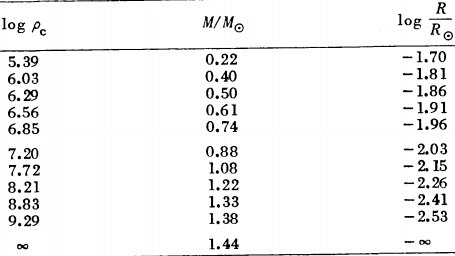
\includegraphics[width=(\textwidth),height=(\textheight-11mm),keepaspectratio]{MRWD}
\caption{Mass/radius relation for completely degenerate WD.}
\end{figure}

\subsection{Limite superiore per la massa di una stella completamente degenere}

Quantit\'a che influenzano l'equilibrio idrostatico:
\begin{align*}
\rho\propto\frac{M}{R^3}&\intertext{questa sopra \'e la densit\'a, questa sotto l'attrazione gravitazionale}\\
\rho\frac{GM_r}{r^2}\propto\frac{M^2}{R^5}
\end{align*}

Per la pressione:
\begin{align*}
P\propto\rho^{\frac{5}{3}}\propto\frac{M^{\frac{5}{3}}}{R^5}&\intertext{per stelle meno massive ho la pressione NR (sopra), per stelle massive uso la formula R (sotto)}\\
P\propto\rho^{\frac{4}{3}}\propto\frac{M^{\frac{4}{3}}}{R^4}
\end{align*}

il cui gradiente genera una forza di pressione
\begin{align*}
F_P&\propto\frac{M^{\frac{5}{3}}}{R^6}\quad\text{NR-D}\\
&\frac{M^{\frac{4}{3}}}{R^5}\quad\text{R-D}
\end{align*}

Osservazioni:
\begin{itemize*}
\item In the relativistic case gravitational force and pressure force depend on the same power of radius.
\item In R-D the 2 forces depend on different power of mass.
\end{itemize*}

\subsection{Massa di Chandrasekhar}

La densit\'a centrale di una nana bianca aumenta come $M^2$ fino all'istaurarsi del regime ultra-relativistico: in regime UR solo una massa \'e in equilibrio.

Usando un modello politropico ricavo
\begin{align*}
M_{Ch}=(\frac{2}{\mu_e})^2*1.459\msun&\intertext{Per nane bianche di He o C ho $\downarrow$}\\
M_{Ch}=1.4\msun
\end{align*}

Per una stella omogenea il T. del viriale ci dice
\begin{align*}
2\int\epsilon_{Cin}\,dV=\frac{3}{5}\frac{GM^2}{R}=\frac{3}{5}G(\frac{4\pi}{3})^{\frac{1}{3}}M^{\frac{5}{3}}\rho^{\frac{1}{3}}
\end{align*}

Nel caso non relativistico

\begin{align*}
&\frac{3}{5}G(3\pi^2)^{\frac{2}{3}}\frac{\hbar^2}{m_e}(\frac{1}{\mu_em_P})^{\frac{5}{3}}M\rho^{\frac{2}{3}}&\intertext{$\mu_e$ \'e il peso molecolare medio quando si considera il contributo alla pressione del gas solo degli elettroni: $\mu_e=1$ per $^1H$, $\mu_e\approx2$ per altri casi($\geq2$ adroni per elettrone). Ho usato $\downarrow$}\\
&P=\frac{1}{20}(\frac{3}{\pi})^{\frac{2}{3}}\frac{h^2}{m_e}n_e^{\frac{5}{3}}=\frac{1}{20}(\frac{3}{\pi})^{\frac{2}{3}}\frac{h^2}{m_em_u^{\frac{5}{3}}}(\frac{\rho}{\mu_e})^{\frac{5}{3}}\\
&=1.0036*10^{13}(\frac{\rho}{\mu_e})^{\frac{5}{3}}\quad(cgs)\\
&P=\frac{2}{3}U_e
\end{align*}

\begin{align*}
\rho\propto G^3(\mu_em_P)^5m_e^3M^2
\end{align*}

Nel caso relativistico

\begin{align*}
M\propto(\frac{c\hbar}{G})^{\frac{3}{2}}\frac{1}{\mu_e^2m_P^2}\to M_{Ch}
\end{align*}

\subsection{WD oscillations.}

Prendendo $\Delta R\approx1\%$:
\begin{equation*}
\Delta E_{grav}\propto \frac{GM^2}{R}\frac{\Delta R}{R}\approx\SI{e48}{\erg}
\end{equation*}

\section{Stelle di neutroni}

\subsection{Formazione}

Nascono dal collasso di una stella ed hanno $T\geq10^{10}\,K$: rapidamente la temperatura della stella diminuisce a causa del flusso di neutrini. In 100 yr $T\approx10^8$, che pu\'o essere considerata bassa vista l'energia massima dei neutroni altamente degeneri:
\begin{align*}
KT\approx10\,KeV\\
E_F\approx1000\,MeV
\end{align*}
L'equazione di stato \'e essenzialmente la stessa che per $T\approx0$.

\subsection{Neutronizzazione}

L'aumento della densit\'a aumenta l'energia degli elettroni che danno luogo con i protoni a electron capture. I nuclei arricchiti di neutroni ($^{118}Kr$) cominciano ad emetterli a una densit\'a $\rho_{dr}\approx4*10^{11}g/cm^3$.\index{Neutron drip}

In questo stadio la materia \'e composta da nuclei (di solito organizzati in reticolo), elettroni e neutroni liberi: il numero di elettroni aumenta con la densit\'a e cos\'i $P_n$.

\begin{align*}
P\approx P_e\gg P_n&\intertext{$\uparrow$ per $\rho\approx\rho_{dr}$}\\
p_n\approx\frac{P}{2}&\intertext{$\uparrow$ per $\rho\approx10^{12}gr/cm^3$}
\end{align*}

\subsection{Fasi successive: Hyperionizzation.}

A partire dall densit\'a per cui i nuclei sono in contatto $\rho_{Nuc}\approx2.4*10^{14}gr/cm^3$ ho un gas/liquido di neutroni degeneri in equilibrio con piccola frazione di \Pproton, \Pelectron: $\Pneutron\leftrightarrow\Pproton+\Pelectron$. 

Successivamente ho iperionizzazione e quark liberi.

\subsection{Massa limite per stelle di neutroni}

Uso i conti fatti per le nane bianche con opportuno scaling

\begin{align*}
m_e\to m_n\\
\underbrace{\mu_{WD}}_2\to\underbrace{\mu_{NS}}_1\\
\end{align*}

ottengo

\begin{align*}
&\rho^{NS}(M)=\rho^{WD}(M)(\frac{m_n}{m_e})^3(\frac{\mu_{NS}}{\mu_{WD}})^5\\
&\approx2.5*10^8\rho^{WD}(M)\\
&\rho^{NS}(M)\approx2.5*10^{14}(\frac{M}{\msun})^2g/cm^3
\end{align*}

e per la massa limite di una stella di neutroni ottengo
\begin{equation*}
M_{Cha}^{NS}=M_{Cha}(\frac{\mu_{WD}}{\mu_{NS}})^2\approx5.7\msun
\end{equation*}
Calcoli pi\'u precisi abbassano il limite?

\section{Buchi neri}

\subsection{Raggio di Schwarzschild}

Alla superficie di una configurazione di massa M e raggio R la curvatura gaussiana dello spazio \'e 
\begin{align*}
&K_G=\frac{GM}{c^2R^3}=-\frac{1}{2}\frac{r_s}{R}\frac{1}{R^2}&\intertext{\'e solitamente piccolo rispetto alla curvatura $R^{-2}$ della superficie sferica:}\\
&-K\approx2*10^{-6}\frac{1}{R^2}&\intertext{$\uparrow$ at surface of the sun}\\
&-K\approx0.15\frac{1}{R^2}&\intertext{$\uparrow$ for neutron star}\\
&-K\approx\frac{1}{R^2}&\intertext{$\uparrow$ for black hole with $R=r_s$}
\end{align*}

Il parametro critico \'e il raggio di Schwarzschild
\begin{equation*}
r_s=\frac{2MG}{c^2}
\end{equation*}
cio\'e la distanza dal centro di attrazione di una massa per cui $v_f=c$.

\subsection{Densit\'a critica}

In termini di densit\'a ho
\begin{align*}
\rho_{Crit}\approx2*10^{16}(\frac{\msun}{M})^2g/cm^3
\end{align*}